\documentclass{article}

\usepackage{amsmath, amsthm, amssymb, amsfonts}
\usepackage{thmtools}
\usepackage{graphicx}
\usepackage{setspace}
\usepackage{geometry}
\usepackage{float}
\usepackage{hyperref}
\usepackage[utf8]{inputenc}
\usepackage[serbian]{babel}
\usepackage{framed}
\usepackage[dvipsnames]{xcolor}
\usepackage{tcolorbox}

\colorlet{LightGray}{White!90!Periwinkle}
\colorlet{LightOrange}{Orange!15}
\colorlet{LightGreen}{Green!15}

\newcommand{\HRule}[1]{\rule{\linewidth}{#1}}

\declaretheoremstyle[name=Theorem,]{thmsty}
\declaretheorem[style=thmsty,numberwithin=section]{theorem}
\tcolorboxenvironment{theorem}{colback=LightGray}

\declaretheoremstyle[name=Proposition,]{prosty}
\declaretheorem[style=prosty,numberlike=theorem]{proposition}
\tcolorboxenvironment{proposition}{colback=LightOrange}

\declaretheoremstyle[name=Principle,]{prcpsty}
\declaretheorem[style=prcpsty,numberlike=theorem]{principle}
\tcolorboxenvironment{principle}{colback=LightGreen}

\setstretch{1.2}
\geometry{
    textheight=9in,
    textwidth=5.5in,
    top=1in,
    headheight=12pt,
    headsep=25pt,
    footskip=30pt
}

% ------------------------------------------------------------------------------

\begin{document}

% ------------------------------------------------------------------------------
% Cover Page and ToC
% ------------------------------------------------------------------------------

\title{ \normalsize \textsc{}
		\\ [2.0cm]
		\HRule{1.5pt} \\
		\LARGE \textbf{\uppercase{Da li bi znanje trebalo da bude besplatno?}
		\HRule{2.0pt} \\ [0.6cm] \LARGE{Predmet: Računarstvo i društvo} \vspace*{10\baselineskip}}
		}
\date{}

\author{\textbf{Darko Zorić 225/2017} \\ 
		Matematički fakultet \\
		2023/2024}

\maketitle
\newpage

\tableofcontents
\newpage

% ------------------------------------------------------------------------------

% ------------------------------------------------------------------------------
% Uvod
% ------------------------------------------------------------------------------

\section{Uvod}

Pitanje da li bi znanje trebalo da bude besplatno je složeno i kontroverzno, posebno kada se razmatraju potencijalno komercijalno vredni konteksti kao što su udžbenici, autorska prava i patenti.

Veliki deo naučnih istraživanja objavljenih u komercijalnim časopisima finansiraju poreski obveznici ili neprofitne institucije i organizacije. Mnogi tvrde da je nepravedno da se ova javno finansirana istraživanja zaključavaju iza različitih vidova plaćanja.

Sa jedne strane, postoji snažan argument za demokratizaciju znanja, sa naglaskom na jednak pristup obrazovnim materijalima i informacijama, dok sa druge strane, postoje opravdane zabrinutosti u vezi sa ekonomskim podsticajima za stvaranje i širenje znanja.

Zastupnici ideje da znanje treba da bude besplatno tvrde da neometan pristup informacijama predstavlja osnovno ljudsko pravo. Obrazovanje je ključni pokretač društvenog i ekonomskog napretka, a pružanje besplatnog pristupa udžbenicima i obrazovnim resursima može pomoći da se izjednače šanse, omogućavajući onima sa ograničenim finansijskim sredstvima da steknu znanje i veštine. Uklanjanjem prepreka za pristup, promovišemo jednakost mogućnosti i smanjujemo nejednakosti u obrazovanju.

Iako je ovo pitanje i dalje predmet rasprave, sve više univerziteta i istraživača podržava otvoreni pristup znanju. Inicijative kao što su masovni otvoreni onlajn kursevi (eng. Massive Open Online Courses - MOOC) i resursi za otvoreno obrazovanje (eng. Open Educational Resources - OER) omogućavaju širenje naučno utemeljenog i odobrenog znanja većem broju zainteresovanih korisnika. Finansijski je takođe održivo u potpunosti dati slobodu pristupa znanju, ili bar omogućiti veći stepen slobode u njegovom korišćenju. Na primer, Harvard je ostvario uštedu od 3,5 miliona dolara godišnje prelaskom na otvorene licence i objavljivanje istraživanja.

% ------------------------------------------------------------------------------
% Kratak istorijski pregled
% ------------------------------------------------------------------------------

\section{Kratak istorijski pregled}

Uspeh homo sapiens-a, predmet razmatranja brojnih kulturologa i antropologa, manje proizlazi iz karakteristika koje nas čine vrhunskim primatima, već više iz našeg talenta za prenošenje znanja kroz vreme. Dobijamo smernice od naših predaka, čuvamo ih i obogaćujemo za buduće generacije.

Zarobljeni u neprijateljskim okruženjima, zapadni istraživači su umirali od gladi, smrzavali se i propadali, dok su domoroci, koje su etiketirali kao divljake, uspevali bez problema. Lišeni lokalnih veština i znanja, iako dobro opremljeni, istraživači nisu uspevali da se prilagode okolini. Lokalno stanovništvo je koristilo svoje "akumulirane baze znanja" da bi pravilno sakupljalo biljke, činilo ih bezopasnim i hranljivim, lovilo tamo gde je bilo najviše divljači i zaštitilo se od prirodnih nepogoda. Kako je ta mreža znanja postajala obimnija i starija, tako su bolje savladavali gotovo svaku situaciju. S druge strane, ti domorodački narodi su gubili veštine kada bi njihova populacija bila smanjena usled drugih napada ili bolesti, a time bi se izgubio i prenos znanja na ostale. Što je više ljudi, veća je i baza akumuliranog znanja i šira je mreža, ali sama brojnost ne garantuje automatski dublje razumevanje.

Sedamdeset hiljada Firentinaca doprinelo je renesansi, dok je pedeset hiljada Edinburžana doprinelo škotskom prosvetiteljstvu. Oni koji žele postići nešto moraju biti dobro obrazovani i obučeni. Pre svega, moraju biti povezani i učiti jedni od drugih.

Pre industrijske revolucije, tehnološki napredak dolazio je u kratkim naletima, retko generišući dugoročni rast ili razvoj. Kontinuirani i održivi napredak postao je moguć tek kada je skup naučnih saznanja produbljen, pokrećući ekonomski korisne akcije. Koliko god specifičan sadržaj znanja bio važan, omogućavanje širokog pristupa pronalazačima i preduzetnicima bilo je podjednako ključno. To je postalo uobičajeno između naučne i industrijske revolucije. Ako znanje nije široko dostupno, ostaje ezoterično i beskorisno.

Biblioteke su simbol našeg kolektivnog uma. Iako ih je internet nadmašio, u analognom dobu bile su najveće akumulacije informacija na jednom mestu. Aleksandrijska biblioteka pod Ptolomejskom vlašću težila je sakupljanju svega što je bilo poznato. Njena ambicija bila je potpuna pokrivenost svega što je ikada napisano. Često je posedovala originalne rukopise, koliko god je to bilo moguće. Ptolomejci su naredili da se kopiraju svi radovi na brodovima koji su prolazili kroz luku Aleksandrije, zadržavajući original, a vraćajući kopiju. Do prvog veka pre nove ere, biblioteka je sakupila 700.000 svitaka, odnosno oko 100.000 dela. Neki od najboljih kartografa i etnografa u drevnom svetu proizveli su naučnici koji nikada nisu izašli van zidova biblioteke. Danas, dok se digitalno doba širi, biblioteke i dalje igraju ključnu ulogu u pristupu informacijama i obrazovanju.

Nedavno je moć umreženog znanja demonstrirana brzinom kojom su istraživači genetski sekvencirali virus SARS-CoV-2 (poznatiji kao COVID-19) 2020. godine. U periodu od 2002. do 2003. godine, sekvenciranje SARS virusa zahtevalo je nekoliko meseci, dok je COVID-19 sekvenciran za samo nekoliko nedelja. Ranije su podaci bili čuvani zarad objavljivanja u prestižnim časopisima koji su naplaćivali pristup. Čak i tokom epidemija ebole i zika virusa, naučne informacije su se kretale sporo. Tokom pandemije 2020. godine, sve prepreke su pale. Kineski istraživači brzo su objavljivali epidemiološke podatke na internetu, omogućavajući njihovu efikasnu upotrebu.

Danas, internet i digitalne platforme omogućavaju trenutno deljenje informacija širom sveta. Ovim je omogućen pristup obimnim bazama podataka, veb stranicama, onlajn kursevima, e-knjigama i drugim resursima koji sadrže veliku količinu informacija. Sajtovi kao što su veb forumi, društvene mreže, blogovi i platforme za razmenu sadržaja omogućavaju korisnicima da postavljaju pitanja, dele svoje znanje, iskustva i ideje, kao i da odgovaraju na pitanja drugih korisnika.

% ------------------------------------------------------------------------------
% Pregled trenutnog znanja: dostupnost i ograničenja
% ------------------------------------------------------------------------------

\section{Pregled trenutnog znanja: dostupnost i ograničenja}

U današnjem svetu, znanje je postalo sveprisutno i dostupno na dohvat ruke zahvaljujući tehnološkom napretku. Međutim, iako je znanje široko dostupno, postoje i određena ograničenja koja utiču na njegovu dostupnost i upotrebu.

Prva stvar koju treba uzeti u obzir jeste da, iako je znanje dostupno, njegov kvalitet može da varira. Na primer, informacije na internetu mogu biti tačne, ali isto tako mogu biti neprecizne, zastarele, a čak i pogrešne. Stoga je važno razumeti kako proceniti kvalitet dostupnih informacija.

Drugo, postoji pitanje pristupa znanju. Iako je tehnologija omogućila široku dostupnost informacija, neki ljudi i dalje nemaju pristup ovim resursima. Ovo može biti rezultat ekonomskih, geografskih ili socijalnih prepreka.

Treće, postoji pitanje upotrebe znanja. Čak i kada je znanje dostupno, neki ljudi možda neće biti u stanju da ga efikasno iskoriste. Ovo može biti rezultat nedostatka obrazovanja ili veština potrebnih za razumevanje i primenu znanja.

Četvrto, postoji pitanje zaštite intelektualne svojine. Dok neko znanje može biti slobodno dostupno, drugo može biti zaštićeno autorskim pravima, patentima i licencama. Ovo može ograničiti širenje i upotrebu ovog znanja.

\begin{figure}[htbp]
    \center
    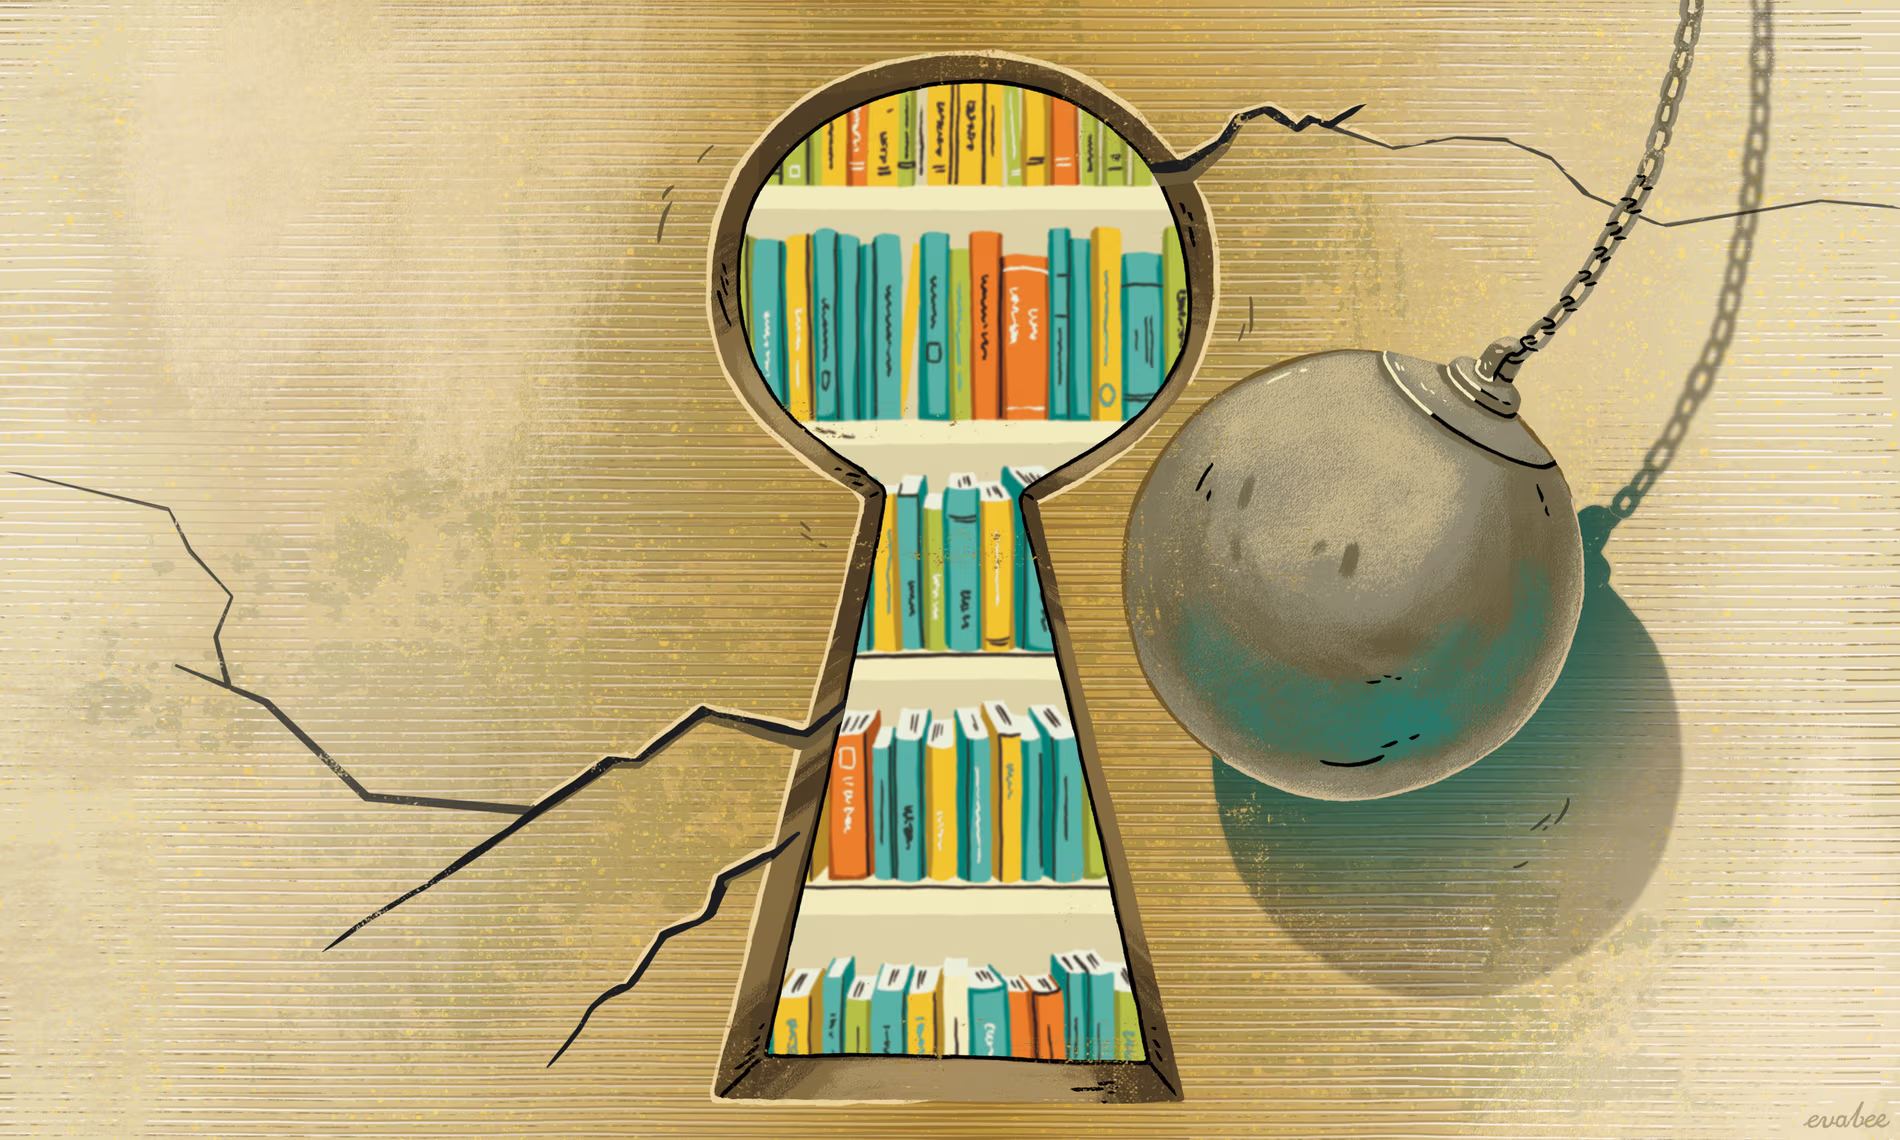
\includegraphics[scale=0.2]{img/lock.png}
    \caption{Danas ne možemo uvek imati direktan pritup znanju}
\end{figure}

Na kraju, postoji pitanje etike u vezi sa korišćenjem i širenjem znanja. Na primer, neke informacije mogu biti osetljive ili privatne, a njihovo neovlašćeno širenje može predstavljati kršenje privatnosti.

U Srbiji postoji fondacija pod nazivom Alek Kavčič, čiji je cilj da reši većinu ovih problema. Njen osnivač je prof. Aleksandar Kavčić, inženjer i naučnik. Kroz svoje aktivnosti, fondacija snažno podržava ideju da znanje treba da bude besplatno i dostupno svima. Ona prepoznaje da pristup obrazovanju i znanju nije privilegija koja bi trebalo da bude rezervisana samo za odabrane, već temeljno pravo koje treba da bude dostupno svima, bez obzira na socioekonomske okolnosti. Jedan od načina na koji Fondacija Alek Kavčič ostvaruje ovu ideju jeste kroz besplatne udžbenike za učenike osnovnih škola.

% ------------------------------------------------------------------------------
% Elsevier
% ------------------------------------------------------------------------------

\section{Elsevier}

Elsevier je globalna izdavačka kompanija koja se bavi distribucijom naučnih, tehničkih i medicinskih sadržaja. Osnovana je 1880. godine i danas je jedan od najvećih i najpoznatijih izdavača naučnih časopisa i akademskih knjiga. Kompanija Elsevier je poznata po svom širokom spektru publikacija u oblastima kao što su medicina, prirodne nauke, inženjerstvo, tehnologija, društvene nauke i humanističke discipline.

Elsevier izdaje preko 2.500 naučnih časopisa, uključujući neke od najuglednijih u svetu nauke, kao što su „The Lancet“ i „Cell“. Pored toga, kompanija takođe objavljuje veliki broj akademskih knjiga, referentnih radova, baza podataka i alata za istraživanje.

\begin{figure}[htbp]
    \center
    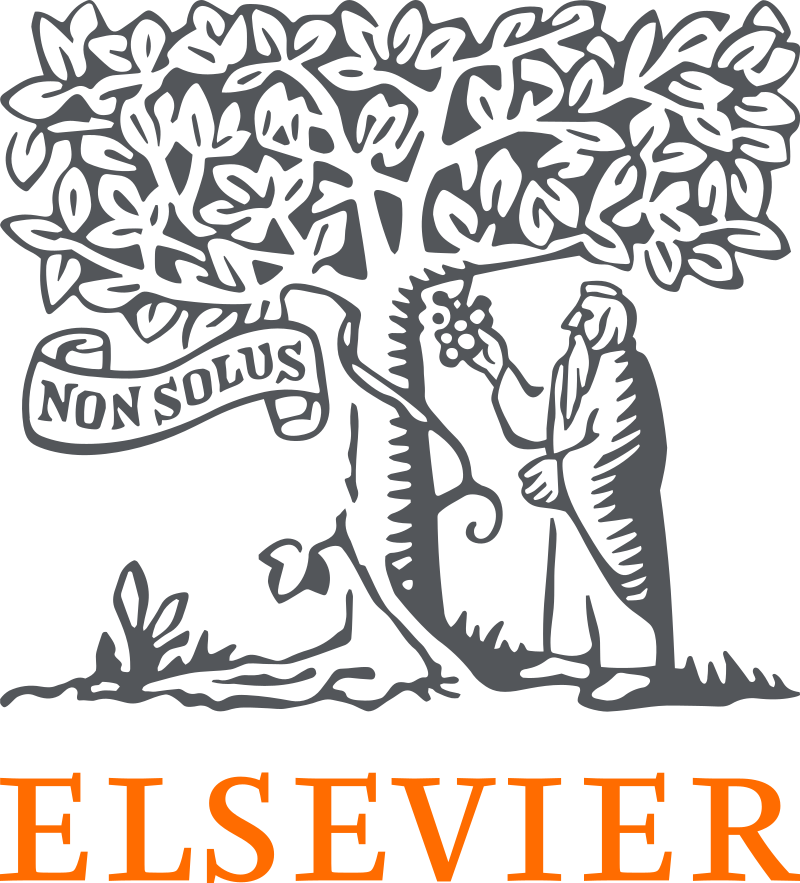
\includegraphics[scale=0.15]{img/elsevier-logo.png}
    \caption{Elsevier logo}
\end{figure}

Međutim, Elsevier je često kritikovan zbog visokih cena svojih časopisa i pristupa koji često ograničava širenje znanja. Neki smatraju da model pretplate na časopise otežava pristup informacijama široj javnosti, posebno u zemljama u razvoju, gde su pristupne takve informacije često ograničene finansijskim sredstvima. On je pokušao da opravda svoje cene kroz naredne argumente:

\begin{enumerate}
    \item Troškovi produkcije i kvalitet: Izdavanje naučnih radova zahteva značajne resurse u smislu uređivanja, recenziranja, dizajna i distribucije. Elsevier tvrdi da visoke cene reflektuju ove troškove, kao i kvalitet rada koji nude. Njihovi časopisi obično prolaze kroz rigorozan proces recenzije kako bi se osigurala visoka naučna i metodološka validnost.
    \item Investicije u istraživanje i razvoj: Izdavači kao što je Elsevier tvrde da deo prihoda od prodaje ide nazad u naučne zajednice kroz finansiranje novih istraživanja i razvoj novih tehnologija za objavljivanje i distribuciju naučnih sadržaja.
    \item Vrednost dodata uslugama: Pored samih naučnih radova, izdavači često pružaju dodatne usluge kao što su alati za analizu podataka, platforme za povezivanje istraživača i visoko kvalitetne baze podataka. Ove usluge dodaju vrednost pretplati i mogu opravdati više cene.
    \item Održavanje kvaliteta i integriteta naučnih izdanja: Elsevier ističe da visoke cene časopisa omogućavaju održavanje visokih standarda kvaliteta i integriteta u procesu izdavanja, uključujući i podršku za recenzente, urednike i druge stručnjake koji učestvuju u kreiranju naučnih izdanja.
    \item Pristup raznovrsnim sadržajima: Pretplata na naučne časopise omogućava pristup širokom spektru istraživanja u različitim disciplinama, što može biti korisno za istraživače koji se bave interdisciplinarnim ili multidisciplinarnim temama.
\end{enumerate}

Kritičari tvrde da ovi argumenti nisu dovoljni da opravdaju visoke cene i zatvoren pristup naučnim radovima, naročito u digitalnom dobu gde je distribucija informacija efikasnija i jeftinija nego ikad.

% ------------------------------------------------------------------------------
% The Cost of Knowledge: Borba Akademika Protiv Elsevier-a
% ------------------------------------------------------------------------------

\section{The Cost of Knowledge: Borba Akademika Protiv Elsevier-a}

"The Cost of Knowledge" protest, pokrenut 2012. godine od strane akademskih istraživača kao odgovor na visoke cene i restriktivne prakse velikih izdavačkih kuća poput Elsevier-a, ima za cilj da podstakne promene u načinu distribucije naučnih radova i da istakne probleme s kojima se suočavaju istraživači.

\begin{figure}[htbp]
    \center
    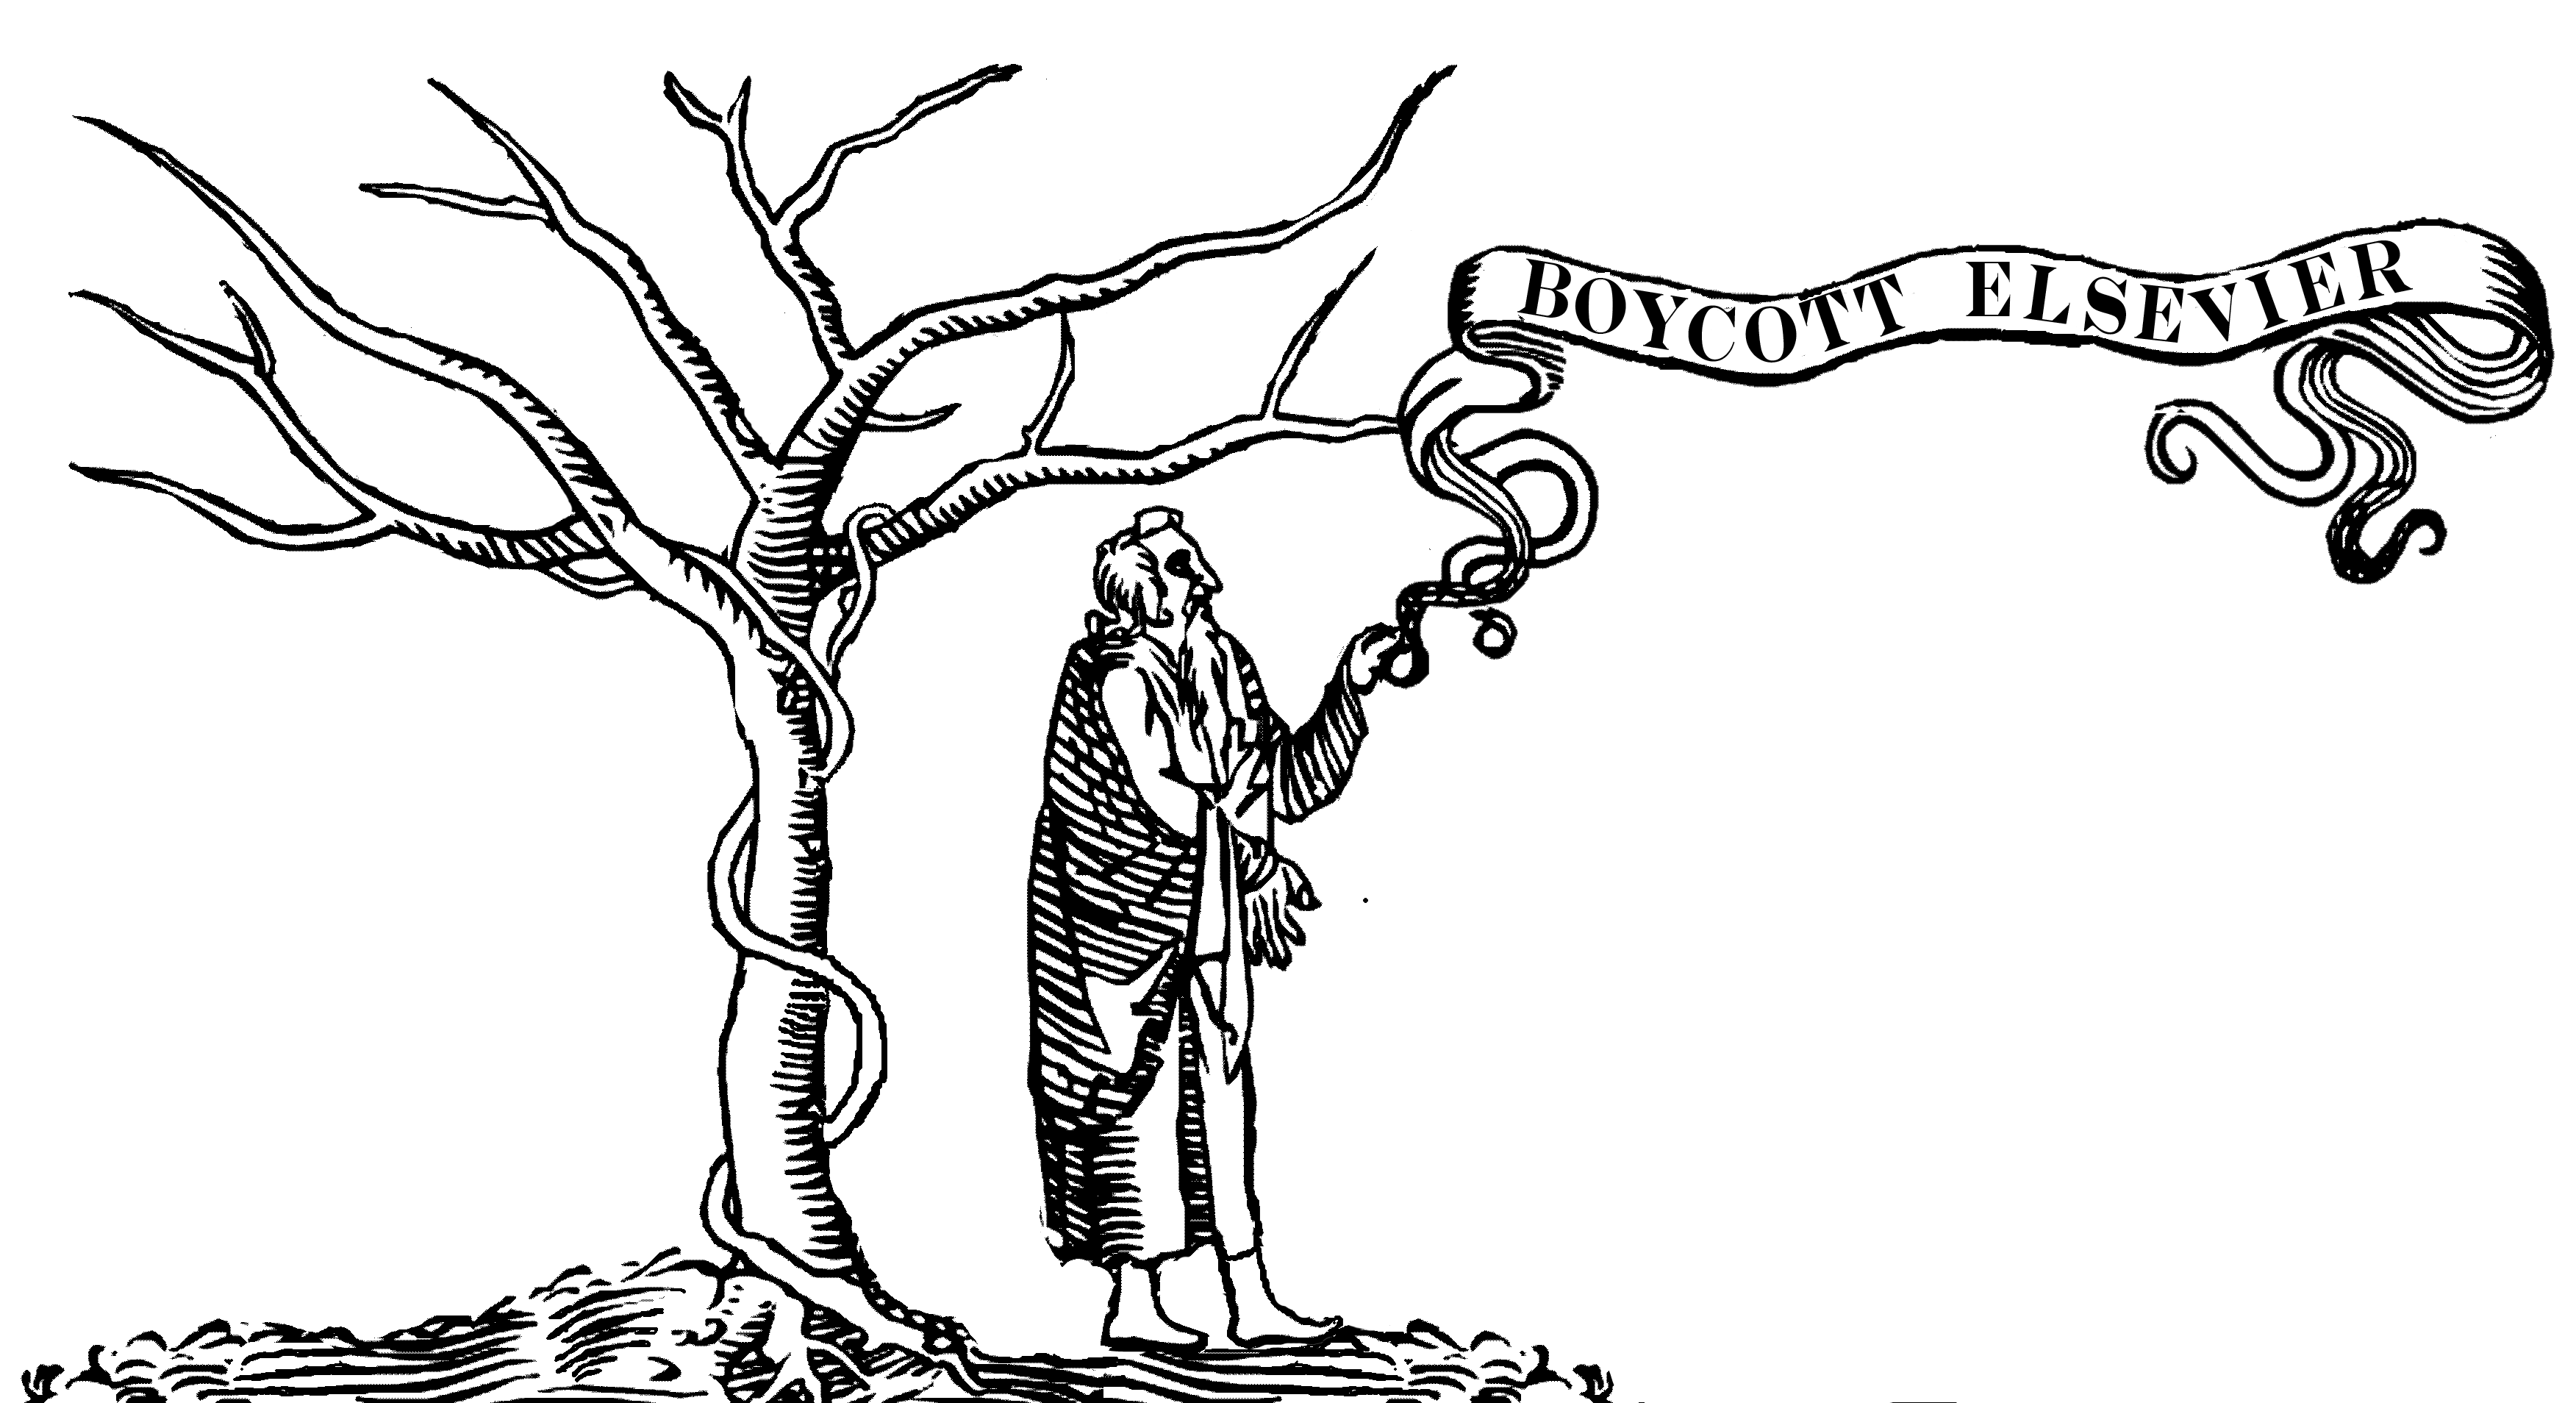
\includegraphics[scale=0.1]{img/Boycott_Elsevier.png}
    \caption{Protestni pokret protiv izdavačke kuće Elsevier}
\end{figure}

Elsevier, kao jedan od najvećih izdavača naučnih radova, često je bio kritikovan zbog visokih cena i restriktivnih politika pristupa informacijama. "The Cost of Knowledge" protest je nastao kao odgovor na ove prakse. Akademski istraživači odlučili su da se udruže i bojkotuju Elsevier-ove časopise kako bi izrazili svoje nezadovoljstvo i zahtevali promene. Pojavila se peticija koja zagovara obustavu saradnje s Elsevier-om, poput prekida slanja radova na njihove časopise, nerecenziranja članaka u njihovim časopisima i neučestvovanja u uređivačkim odborima. Do februara 2012. godine, ovu peticiju je potpisalo preko 5.000 akademika, a do novembra 2018. godine preko 17.000.

Glavni argumenti protiv Elsevier-a i sličnih izdavača su da visoke cene pretplata otežavaju pristup naučnim radovima, posebno za istraživače u zemljama s manjim budžetima za istraživanje. Takođe, mnogi istraživači su frustrirani restrikcijama vezanim za autorska prava i distribuciju svojih radova, što kao posledicu ima ograničavanje širenja znanja.

Bojkot Elsevier-a sastoji se od nekoliko glavnih akcija. Istraživači odbijaju objavljivati svoje radove u Elsevier-ovim časopisima, otkazuju pretplate na ove časopise i pozivaju druge istraživače da im se pridruže. Takođe su se organizovali da pruže podršku alternativnim modelima izdavanja i distribucije naučnih radova, poput otvorenog pristupa (eng. Open Access) publikacijama.

Rezultati protesta su bili raznoliki. S jedne strane, Elsevier se suočio s javnim pritiskom i kritikama, što je dovelo do nekih promena u njihovim politikama, kao što su olakšavanje pristupa naučnim arhivama ili fleksibilniji uslovi autorskih prava. S druge strane, protest nije doveo do potpunog preokreta u industriji izdavaštva naučnih radova, a neki istraživači i dalje su nastavili objavljivati u Elsevier-ovim časopisima.

Ipak, "The Cost of Knowledge" protest imao je dalekosežne posledice. Pokrenuo je širu raspravu o pravima istraživača, održivosti izdavačkih modela i potrebi za otvorenijim pristupom naučnim informacijama. Pored toga, inspirisao je druge slične inicijative i podstakao razvoj alternativnih modela izdavanja koji su više usmereni ka otvorenom pristupu znanju.

% ------------------------------------------------------------------------------
% Sci-Hub
% ------------------------------------------------------------------------------

\section{Sci-Hub}

U digitalnom dobu, pristup naučnim radovima predstavlja ključni faktor u razvoju nauke i obrazovanja. Međutim, ograničenja koja postavljaju visoke cene časopisa i zaključana prava pristupa predstavljaju prepreke za mnoge istraživače, studente i akademike. U tom kontekstu, Sci-Hub, platforma koja omogućava besplatan pristup naučnim radovima, postala je ključna figura u borbi za otvoren pristup znanju.

\begin{figure}
    \centering
    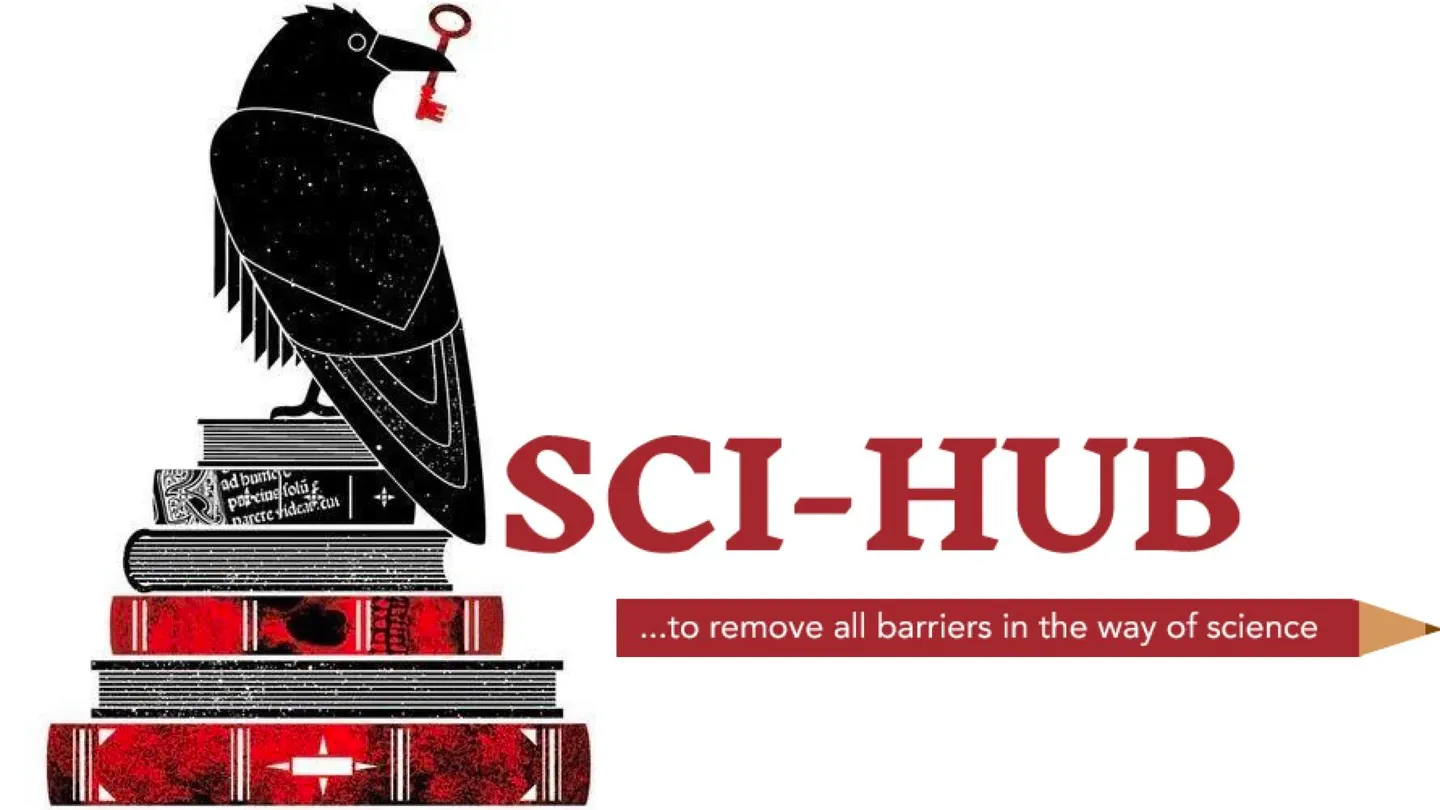
\includegraphics[width=0.75\linewidth]{img/sci-hub.png}
    \caption{Sci-Hub - besplatna platforma za pristup akademskim i naučnim radovima}
\end{figure}

Sci-Hub je osnovan 5. septembra 2011. godine od strane neurobiologa Aleksandre Elbakijan, sa ciljem da omogući besplatan pristup naučnim radovima širom sveta. Aleksandra Elbakijan (koja je dobila nadimak „Robin Hud nauke“) započela je ovaj projekat iz frustracije prema visokim cenama naučnih časopisa i ograničenjima pristupa koji su mnogima onemogućavali da prate najnovija istraživanja. Sci-Hub funkcioniše tako što omogućava korisnicima da preuzimaju naučne radove sa velikog broja izvora, često bez dozvole izdavača. Ovaj sistem je postao izuzetno popularan, naročito među studentima i istraživačima iz zemalja sa manjim i ograničenim budžetima za istraživanje. Danas se na njemu nalazi preko 85 miliona radova.

Jedan od najznačajnijih aspekata Sci-Hub-a je što omogućava širok pristup naučnim radovima koji su inače nedostupni zbog visokih cena ili pretplate na određene časopise. Ovo je naročito važno u zemljama u razvoju gde su bibliotečki resursi ograničeni, a troškovi pristupa časopisima su često ogromni. Sci-Hub pomaže istraživačima da prate najnovija dostignuća u svojim oblastima, što može značajno unaprediti kvalitet naučnih radova i doprineti bržem napretku u različitim disciplinama.

Međutim, Sci-Hub nije mogao da prođe bez kontroverzi. Naime, Elsevier je 2015. godine podneo tužbu protiv Sci-Hub-a. To je bio najveći slučaj kršenja autorskih prava koji je u to vreme podnet u SAD ili u svetu. Elsevier je tražio novčanu odštetu i zabranu da zaustavi deljenje naučnih radova i  koristio je optužbe o navodnoj bezbednosnoj pretnji koju Sci-Hub predstavlja institucijama da podstakne obrazovne institucije da blokiraju njegovu upotrebu. Danas mnogi izdavači smatraju da ovaj sajt nanosi štetu industriji izdavaštva. Oni tvrde da besplatan pristup naučnim radovima oduzima finansijsku podršku izdavačima, što može dovesti do smanjenja kvaliteta usluga i lošije uslove za istraživanje. Takođe, neki ističu da Sci-Hub obezvrednjuje trud naučnika i izdavača, koji ulažu svoje resurse u stvaranje i distribuciju naučnih radova.

\begin{figure}
    \centering
    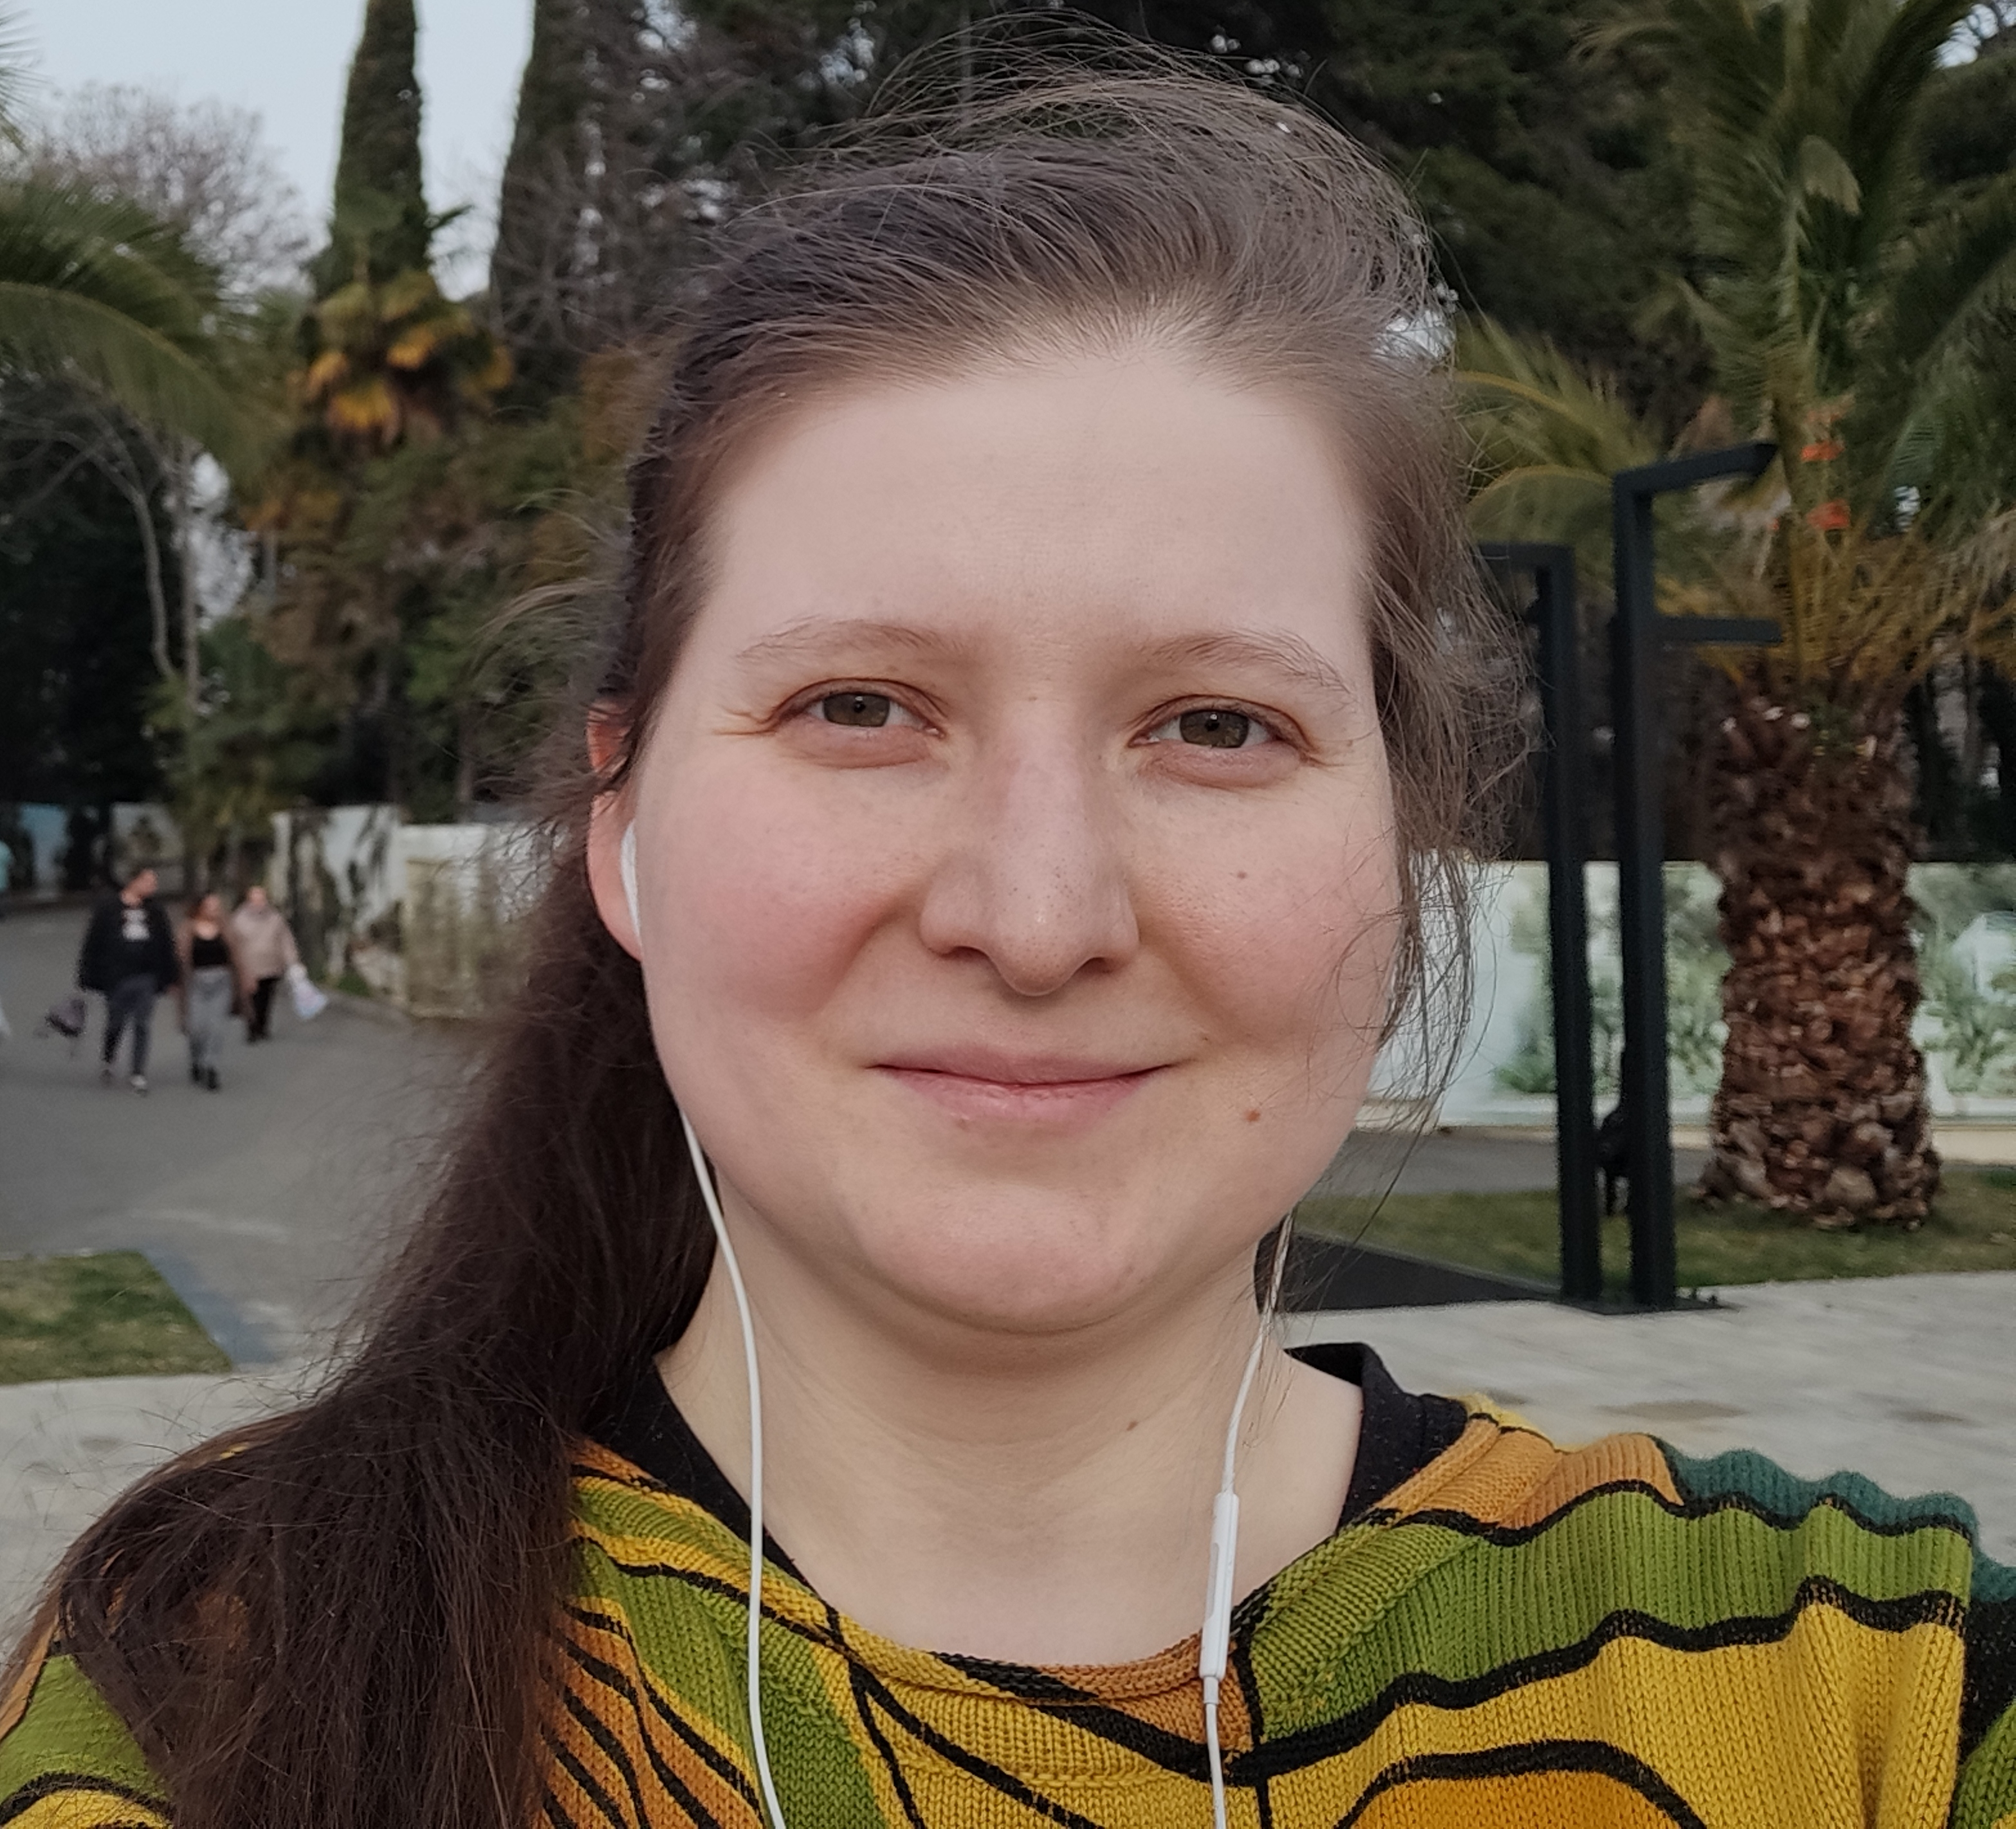
\includegraphics[width=0.5\linewidth]{img/Alexandra_Elbakyan.jpg}
    \caption{Aleksandra Elbakijan, osnivač Sci-Hub-a}
\end{figure}

Pored toga, postoji i pitanje održivosti Sci-Hub-a na duže staze. Platforma se suočava sa pravnim izazovima i pokušajima blokiranja pristupa izdavača. Takođe, finansiranje predstavlja izazov, s obzirom na to da se oslanja uglavnom na donacije i volonterski rad. Dok je Sci-Hub trenutno dostupan, neizvesna budućnost može izazvati zabrinutost među korisnicima o tome da li će ova platforma ostati dostupna u budućnosti.

Studija iz 2023. godine otkrila je da više od 50\% akademskih istraživača koristi veb stranice poput Sci-Hub-a kako bi izbegli plaćanje. Oni koji ne koriste Sci-Hub često su naveli nedostatak informacija o samom sajtu kao glavni razlog zašto ga ne koriste. Druga studija, takođe objavljena 2023. godine, zaključila je da Sci-Hub ima široku upotrebu među studentima i profesorima, čak i na velikim istraživačkim univerzitetima u razvijenim zemljama. Razlozi za to uključuju veću kolekciju istraživačkih članaka u poređenju s bilo kojom bibliotekom u svetu, kao i korisnički interfejs koji je lakši za korišćenje prilikom preuzimanja ovih članaka u poređenju s akademskim bibliotekama. Pored akademskih istraživača, još jedna značajna grupa korisnika Sci-Hub-a su medicinski profesionalci van univerzitetskih bolnica, koji obično nemaju pristup originalnim publikacijama u medicinskim časopisima. Ista studija je otkrila da mlađi istraživači i medicinski radnici češće koriste Sci-Hub u poređenju sa svojim starijim kolegama.

% ------------------------------------------------------------------------------
% Otvoren pristup 
% ------------------------------------------------------------------------------

\section{Otvoreni pristup}

\subsection{Definicija, motivacija i značaj}

Otvoreni pristup (Open Access - OA) predstavlja slobodan, besplatan, neograničen online pristup naučnim radovima, pre svega akademskim člancima, knjigama i disertacijama. Ovaj pokret nastao je kao reakcija na paradoksalnu situaciju u kojoj se rezultati istraživanja, finansirani najčešće sredstvima univerziteta ili instituta, objavljuju u časopisima komercijalnih izdavača na čija izdanja te iste institucije moraju da se pretplate kako bi koristile dobijene rezultate.

Otvoreni pristup prvi put je definisan u Budimpeštanskoj deklaraciji, potpisanoj 2002. godine (Budapest Open Access Initiative). Prema toj deklaraciji, otvoreni pristup podrazumeva da svaki korisnik koji ima pristup internetu može da čita, preuzima, kopira i štampa materijal bez ikakvih tehničkih, pravnih ili finansijskih barijera. Jedina obaveza korisnika je da autoru obezbedi nadzor nad integritetom dela i da delo ispravno citira. Godinu dana kasnije, 2003. godine, objavljena je Berlinska deklaracija o otvorenom pristupu naučnom znanju (Berlin Declaration on Open Access to Knowledge in the Sciences and Humanities), koja označava početak uključivanja istraživačkih organizacija u Pokret za otvoreni pristup. Do danas, ovu deklaraciju potpisalo je više od 300 akademskih institucija u svetu, uključujući Univerzitet u Beogradu i Univerzitet u Nišu, koji su je potpisali u novembru 2011. godine.

\begin{figure}[htbp]
    \center
    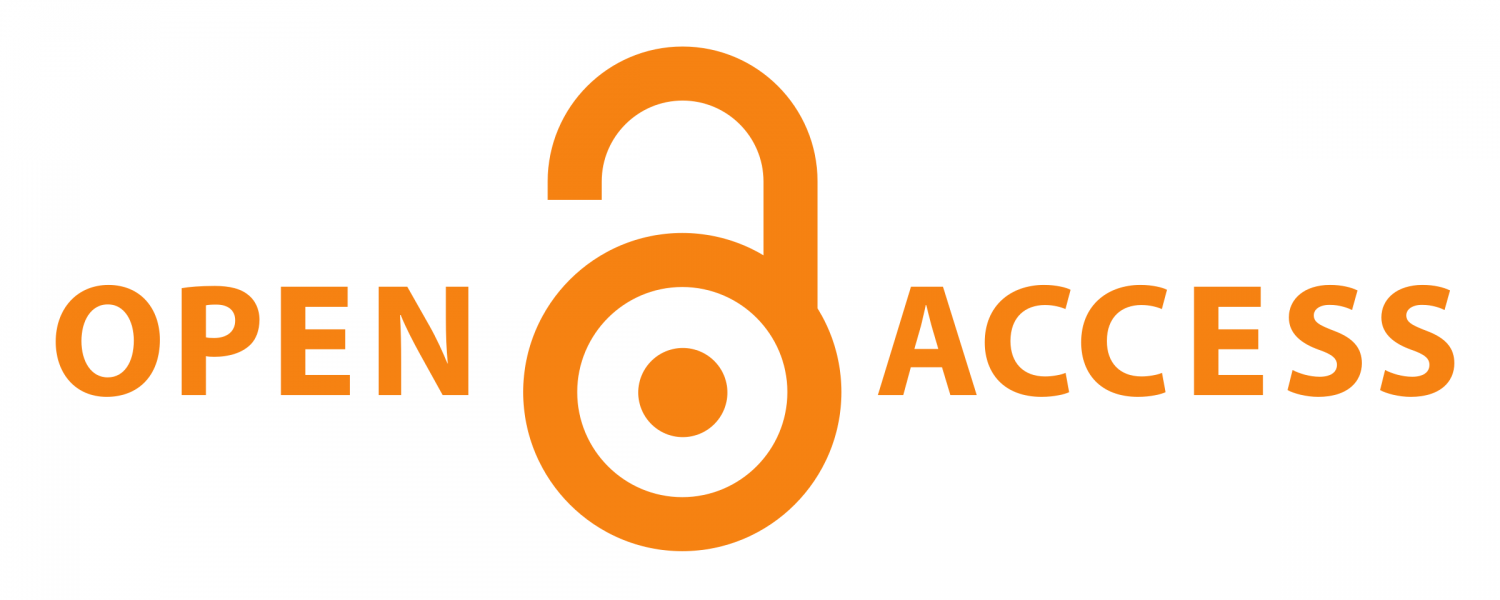
\includegraphics[scale=0.15]{img/open-access-logo.png}
    \caption{Open Access logo}
\end{figure}

\subsection{Osnovni oblici otvorenog pristupa}

Otvoreni pristup ispoljava se kroz dva osnovna oblika:

\begin{itemize}
    \item \textbf{Samoarhiviranje (Self-archiving):} Ovo podrazumeva pohranjivanje verzija radova u digitalne repozitorijume, institucionalne ili tematske – "zeleni put" (green).
    \item \textbf{Časopise u otvorenom pristupu:} Časopisi u potpunosti ili delimično (hibridni časopisi) – "zlatni put" (gold). Troškove objavljivanja u ovakvim časopisima najčešće snose sami autori, dok je pristup člancima besplatan za krajnjeg korisnika.
\end{itemize}

\subsection{Izveštaj Dejm Dženet Finč}

Godine 2012. objavljen je izveštaj autorke Dejm Dženet Finč (Dame Janet Finch), profesorke sociologije na Univerzitetu u Mančesteru, pod nazivom "Accessibility, sustainability, excellence: how to expand access to research publications". U ovom obimnom dokumentu favorizuje se "zlatni put", dok se uloga institucionalnih repozitorijuma svodi na sivu literaturu, odnosno arhiviranje rezultata istraživanja. Izveštaj je vrlo brzo izazvao oštre kritike, naročito među zagovornicima "zelenog puta" kao što je Stiven Harnad (Stevan Harnad). Harnad, koji smatra da je jedini pravi otvoreni pristup onaj koji podrazumeva arhiviranje preprint verzije rada u digitalni repozitorijum, izveštaj je nazvao fijaskom, a svoje tvrdnje je potkrepio pokazateljima racionalnosti i efektivnosti zelenog pristupa. Veliki broj izdavača dopušta autorima da preprint verzije radova pohrane u digitalni repozitorijum svoje institucije. Informacije o politici pojedinih izdavača u vezi sa ovakvim arhiviranjem pruža servis SHERPA/Romeo (Securing a Hybrid Environment for Research Preservation and Access).

\subsection{Digitalni repozitorijumi}

Digitalni repozitorijumi su kolekcije digitalnih objekata, tekstova, slika, video i audio materijala i dr. u odgovarajućem preporučenom formatu. Vrlo često, objekte u repozitorijum unose ovlašćeni korisnici, autori, odnosno nosioci autorskog prava, putem samoarhiviranja, a uneti objekat dobija trajni link kao stalnu adresu na mreži. Repozitorijumi se uglavnom dele na:

\begin{itemize}
    \item Institucionalne, multidisciplinarne, najčešće pri univerzitetima;
    \item Tematske (npr. medicina – PubMed Central, ekonomija – RePEc, matematika, fizika – arXiv);
    \item Poljoprivreda – AgEcon;
    \item Društvene nauke – Social Science Open Access Repository;
    \item Druge specifične oblasti.
\end{itemize}

\subsection{Otvoreni pristup u Srbiji}

\subsubsection{Bibliografske baze podataka i nacionalni citatni indeks}

Ideja otvorenog pristupa naučnim informacijama u Srbiji razvija se od druge polovine devedesetih godina dvadesetog veka i prvi put je sprovedena u delo u bibliografskoj bazi podataka SocioFakt – jugoslovenskoj bazi za društvene činjenične nauke. Tehnološkim unapređenjem i proširivanjem sadržaja te baze nastali su SocioFakt online, srpski citatni indeks za društvene nauke (2001), i SocioFakt Open Access (2004), koji je sadržao protokol za razmenu metapodataka (OAI-PMH), što je omogućilo njegovu integraciju s bazom Google Scholar. Svoju konačnu formu ovi napori dobili su 2006—2007. godine u SCIndeks-u, nacionalnom citatnom indeksu koji referiše domaće časopise iz svih naučnih oblasti kategorizovane kao periodične publikacije naučnog karaktera, od kojih je gotovo polovina dostupna u vidu punog teksta, a veliki broj radova je u režimu otvorenog pristupa.

\subsubsection{Skupovi o otvorenom pristupu}

Prve konferencije, savetovanja i radionice o otvorenom pristupu u Srbiji održavaju se neposredno nakon definisanja Budimpeštanske inicijative o otvorenom pristupu (2002) i Berlinske deklaracije o otvorenom pristupu znanju u prirodnim i humanističkim naukama (2003) – na primer, The International OA Workshop, međunarodna radionica održana 24. novembra 2003. godine. Na ovom skupu, pored pomenutog problema citatnih baza podataka, tema otvorenog pristupa se proširuje i na naučne časopise. Značajan pomak na tom planu učinjen je 2005. godine uspostavljanjem servisa DOISerbia, repozitorijuma koji sadrži radove iz najznačajnijih naučnih časopisa iz Srbije. Krajem marta 2015. godine ovaj repozitorijum obuhvatao je 66 časopisa i 29197 naučnih članaka u otvorenom pristupu.

Veliki značaj za promovisanje otvorenog pristupa u Srbiji imala je i Međunarodna radionica o citatnim indeksima u otvorenom pristupu, održana 10. i 11. novembra 2005. u Beogradu. Tada su, između ostalih, predavanja održali Žan Pol Gedon i Tim Brodi, rodonačelnici otvorenog pristupa. U isto vreme, u časopisu „Infoteka“ objavljeno je nekoliko članaka o ovoj temi. Posebno je značajan tekst Lilijan Van der Vart o institucionalnim repozitorijumima, kojim se ova tema uvodi u našu sredinu.

\subsubsection{Doktorske teze u otvorenom pristupu}

U novembru 2011. godine Univerzitet u Beogradu potpisao je Berlinsku deklaraciju i tako se pridružio grupi od 340 univerziteta i naučnih ustanova u svetu. Nakon potpisivanja deklaracije, Univerzitet je na svojim stranicama objavio tekst „Otvoreni pristup naučnom znanju“, u kome nastavnicima, istraživačima, saradnicima i studentima preporučuje da kad god je to moguće objavljuju svoje radove u časopisima u otvorenom pristupu. U skladu sa ovom odlukom, iste godine, Univerzitet u Beogradu uspostavio je svoj Digitalni repozitorijum sa otvorenim pristupom u Univerzitetskoj biblioteci „Svetozar Marković“ – PHAIDRA (Permanent Hosting, Archiving and Indexing of Digital Resources and Assets). Naredne godine, u okviru sistema PHAIDRA uspostavljen je sistem E-teze, repozitorijum koji arhivira doktorske disertacije odbranjene na univerzitetima u Beogradu, Nišu i Kragujevcu. Univerzitet u Novom Sadu samostalno razvija digitalnu biblioteku doktorskih disertacija u okviru CRIS UNS sistema.

Godine 2013. pokrenut je servis doiSerbia PhD – nacionalni portal doktorskih disertacija dostupnih u elektronskom formatu. Svakoj disertaciji je dodeljen DOI broj. Ovaj portal sadrži linkove ka punom tekstu disertacija koje se nalaze u univerzitetskim repozitorijumima. Posredstvom protokola za razmenu metapodataka (OAI PMH), metapodatke sa ovog portala preuzima i servis DART Europe Arhivirano na sajtu Wayback Machine (13. septembar 2015) – portal evropskih digitalnih disertacija. Izmenama i dopunama Zakona o visokom obrazovanju iz 2014. godine utvrđuje se obaveza visokoškolske ustanove da doktorsku disertaciju koja se u njoj brani i izveštaj komisije o oceni disertacije učini dostupnim javnosti, i to u elektronskoj verziji na zvaničnoj internet stranici ustanove i u štampanom obliku u biblioteci ustanove, najmanje 30 dana pre usvajanja izveštaja komisije na nadležnom organu, kao i do odbrane disertacije; i obaveza univerziteta da ustanovi digitalni repozitorijum u kojem se trajno čuvaju elektronske verzije odbranjenih doktorskih disertacija, zajedno sa izveštajem komisije za ocenu disertacije, podacima o mentoru, sastavu komisije i podacima o zaštiti autorskih prava, kao i da sve navedene podatke učini javno dostupnim (Član 30 Zakona o visokom obrazovanju). Krajem 2015. godine uspostavljen je NaRDuS - centralni nacionalni repozitorijum doktorskih disertacija koji, pored teza, sadrži i izveštaje komisija o njihovoj oceni.

\subsubsection{Tematski i institucionalni repozitorijumi}

Razvoj tematskih i institucionalnih repozitorijuma u Srbiji još uvek je u povoju. Prema podacima iz međunarodnih registara repozitorijuma otvorenog pristupa OpenDOAR i ROAR, u Srbiji trenutno postoje dva tematska repozitorijuma (eLibrary - posvećen matematici; održavaju ga Matematički fakultet Univerziteta u Beogradu i Matematički institut SANU; softverska platforma: DSpace) i CaSA NaRA (održava ga Poljoprivredni fakultet Univerziteta u Beogradu; DSpace), kao i četiri institucionalna (Digitalni repozitorijum Instituta tehničkih nauka SANU i Digitalni repozitorijum Instituta za filozofiju i društvenu teoriju – kao softversku platformu koriste programski paket otvorenog koda OPUS4; IRIES - Institucionalni repozitorijum radova Instituta ekonomskih nauka (EPrints) i RADaR - institucionalni repozitorijum Instituta za biološka istraživanja „Siniša Stanković“ (DSpace).

\subsubsection{Naučne monografije u otvorenom pristupu}

Iako su naučne monografije znatno ređe dostupne u režimu otvorenog pristupa od naučnih radova objavljenih u časopisima, tokom poslednjih desetak godina, pojedine naučne ustanove u Srbiji (Etnografski institut SANU, Balkanološki institut SANU, Geografski institut „Jovan Cvijić“ SANU, Institut tehničkih nauka SANU itd.) na svojim zvaničnim sajtovima objavljivale su digitalne verzije svojih monografskih izdanja. Polazeći od zapažanja da Partnerski program „Gugl knjige“ može da posluži kao dobra platforma za objavljivanje publikacija u režimu otvorenog pristupa, Sekcija bibliotekara i knjižničara Zajednice instituta Srbije započela je u proleće 2013. godine realizaciju projekta uključivanja izdanja naučnoistraživačkih instituta Srbije u ovaj program. Do jula 2017, preko 300 izdanja naučnih instituta iz Srbije objavljeno je na Gugl knjigama u režimu otvorenog pristupa. Među institucijama koje Partnerski program „Gugl knjige“ koriste za objavljivanje digitalnih verzija svojih izdanja u otvorenom pristupu nalaze se Univerzitetska biblioteka „Svetozar Marković“, Etnografski muzej u Beogradu i Srpska akademija nauka i umetnosti.

\subsubsection{Međunarodna nedelja otvorenog pristupa}

Još jedan značajan korak u promovisanju ideje otvorenog pristupa predstavlja obeležavanje Međunarodne nedelje otvorenog pristupa. U Srbiji je ova međunarodna manifestacija prvi put obeležena 2009. godine svečanom tribinom organizovanom na Medicinskom fakultetu u Beogradu, a od 2012. godine redovno se obeležava tokom poslednje nedelje oktobra u organizaciji Univerzitetske biblioteke „Svetozar Marković“ i partnerskih institucija nizom prigodnih aktivnosti. U okviru obeležavanja Međunarodne nedelje otvorenog pristupa, pojedincima koji su se posebno istakli u promovisanju principa otvorenog pristupa naučnim informacijama dodeljuje se počasno zvanje „Arhont otvorenog pristupa“.

% ------------------------------------------------------------------------------
% Plan S
% ------------------------------------------------------------------------------

\section{Plan S}

"Plan S" je inicijativa koja ima za cilj da transformiše način objavljivanja naučnih istraživanja tako što će omogućiti otvoren pristup (Open Access) svim naučnim publikacijama finansiranim javnim sredstvima. Ovaj plan je prvi put objavljen u septembru 2018. godine i potpisali su ga različiti evropski istraživački fondovi i organizacije, zajedno sa Komisijom Evropske unije.

Glavni cilj "Plan S" je postizanje potpunog otvorenog pristupa naučnim radovima do 2021. godine. To znači da će svi rezultati istraživanja finansiranih javnim sredstvima morati biti odmah dostupni bez ikakvih prepreka ili plaćanja. Ovaj plan obuhvata nekoliko ključnih principa:

\begin{enumerate}
    \item Nijedna naučna publikacija finansirana javnim sredstvima ne sme biti iza plaćene prepreke: To znači da svi naučni radovi moraju biti odmah dostupni u otvorenom pristupu bez ikakvih naknada za čitanje ili preuzimanje.
    \item Autori moraju zadržati autorska prava nad svojim radovima: "Plan S" zahteva da autori zadrže autorska prava nad svojim radovima i omoguće njihovo besplatno preuzimanje i deljenje.
    \item Institucije i istraživački fondovi moraju podržavati otvoreni pristup: Institucije i finansijeri istraživanja moraju aktivno podržavati otvoreni pristup naučnim radovima i promovisati njegovo usvajanje među istraživačima.
    \item Potreba za održivošću modela otvorenog pristupa: "Plan S" naglašava potrebu za razvijanjem održivih poslovnih modela koji podržavaju otvoreni pristup, kako bi se osiguralo da finansiranje istraživanja ostane održivo i da se izbegnu visoke naknade za autore.
\end{enumerate}

Ovaj plan je dobio podršku od mnogih akademskih i istraživačkih zajednica, ali je takođe izazvao i određena negodovanja, posebno u vezi sa finansijskim aspektima i prilagođavanjem izdavačkih modela. Portparol kompanije Elsevier izjavio je: "Ako smatrate da bi informacije trebalo da budu besplatne, idite na Vikipediju."


"Plan S" ostaje ključna inicijativa u promovisanju otvorenog pristupa naučnim radovima i podsticanju transparentnosti i pristupačnosti naučnih informacija.


% ------------------------------------------------------------------------------
% Filozofski pristup
% ------------------------------------------------------------------------------

\section{Filozofski pristup}

Znanje, kao osnovno ljudsko dobro, predstavlja ključnu komponentu razvoja društva i individualnog napretka. Postavlja se pitanje da li bi znanje trebalo da bude besplatno, što otvara široku debatu na filozofskom i etičkom nivou.

Na filozofskom nivou, moralnost pristupa znanju predstavlja suštinsko pitanje. Da li je moralno ograničavati pristup informacijama koje imaju potencijal da promene svet ili je moralnije osigurati da svi imaju jednaku mogućnost pristupa znanju koje je ključno za razvoj ljudskog društva? Ograničavanje pristupa znanju može rezultirati nepravdom i neravnopravnošću, dok njegova široka dostupnost može doprineti inkluzivnijem društvu i većem napretku. 

Za zagovornike besplatnog pristupa znanju, ono je inherentno ljudsko pravo, a ne privilegija koja treba da se zasluži. Svako bi trebao imati pravo na obrazovanje i pristup informacijama bez obzira na materijalni status ili druge faktore. Ovo je posebno važno u današnjem digitalnom dobu, gde tehnologija omogućava brz i lagan pristup informacijama. 

Međutim, sada se postavlja pitanje kako se ovo odražava na prava autora i izdavača. Autorska prava su bitna za očuvanje intelektualne svojine i podsticanje kreativnosti. Besplatan pristup znanju može dovesti do smanjenja prihoda autora i izdavača, što može uticati na kvalitet i obim dostupnih informacija. Nedavno smo bili svedoci sudskih sporova proizašlih iz upotrebe veštačke inteligencije koja se obučavala na materijalu sa autorskim pravima. Većina ljudi podržava koncept autorskih prava u kontekstu stvaranja umetničkih dela kao što su romani, muzika, slike i skulpture, čak i ako se ta prava daju na ograničeno vreme. Međutim, šta je sa divnom jednačinom...
\begin{equation*}
e = mc^2
\end{equation*}
...koju je prvi formulisao Albert Ajnštajn? Da li je mogao da zaštiti autorska prava na nju? Ili da je patentira? Da li bi to uopšte mogao?

Da bi se postigao balans između prava autora i širokog pristupa znanju, neke organizacije zagovaraju modele otvorenog pristupa, gde se informacije dele besplatno, ali se autori i izdavači kompenzuju na druge načine, kao što su subvencije ili sponzorstva. 

U krajnjoj liniji, pitanje da li bi znanje trebalo da bude besplatno zahteva pažljivo balansiranje između prava pojedinaca na obrazovanje i pristup informacijama i prava autora na pravednu kompenzaciju za svoj rad. Moramo težiti društvu u kojem je znanje dostupno svima, ali i poštovati prava i interese onih koji ga stvaraju. Besplatni pristup znanju može biti moralno ispravan cilj, ali samo ako se postigne na način koji poštuje prava i doprinos autora i izdavača.

% ------------------------------------------------------------------------------
% Zaključak
% ------------------------------------------------------------------------------

\section{Zaključak}

U svetu koji se rapidno menja zbog tehnološkog napretka, važno je tražiti održive modele pristupa znanju koji omogućavaju širok pristup, poštuju autorska prava i podržavaju dalji napredak društva i nauke. Besplatni pristup znanju predstavlja ključni element u izgradnji bolje budućnosti, ali mora biti uravnotežen sa potrebom za podrškom istraživačima i autorima.

Demokratizacija znanja zahteva kolektivni napor svih relevantnih učesnika - akademika, istraživača, izdavača, vlade i civilnog društva. Potrebno je uspostaviti dinamičan dijalog i inovativne strategije kako bi se postigla ravnoteža između otvorenog pristupa znanju i očuvanja autorskih prava. 

Kroz ove napore, može se stvoriti svet u kojem je znanje zaista dostupno svima, bez obzira na ekonomske, geografske ili druge barijere. Ovo nije samo pitanje pristupa informacijama, već i pitanje demokratizacije znanja i osnaživanja pojedinaca. 

Jedan od ključnih aspekata ove transformacije je podrška institucijama, kao što su univerziteti i istraživačke organizacije, u uspostavljanju digitalnih repozitorijuma i promociji otvorenog pristupa publikacijama. Takođe je važno raditi na edukaciji autora o prednostima otvorenog pristupa i alternativnim modelima distribucije znanja.

Svako društvo može imati koristi od otvorenog pristupa znanju. To omogućava bržu diseminaciju informacija, podstiče naučni napredak i omogućava inovacije koje mogu rešiti globalne probleme. 

Promocija otvorenog pristupa znanju zahteva globalni angažman i usklađene napore svih relevantnih aktera. Samo kroz dijalog, inovaciju i saradnju može se stvoriti inkluzivno društvo u kojem je znanje dostupno svima, podstičući tako napredak i prosperitet čitavog čovečanstva.


% ------------------------------------------------------------------------------



% ------------------------------------------------------------------------------


% ------------------------------------------------------------------------------


% ------------------------------------------------------------------------------


% ------------------------------------------------------------------------------


% ------------------------------------------------------------------------------


% ------------------------------------------------------------------------------


\newpage

% ------------------------------------------------------------------------------
% Reference and Cited Works
% ------------------------------------------------------------------------------

\bibliographystyle{IEEEtran}
\bibliography{References.bib}

% ------------------------------------------------------------------------------

\end{document}
